\documentclass[a4paper,10pt,twoside,openany]{article}

\usepackage[lang=hebrew]{maths}
\usepackage{hebrewdoc}
\usepackage{stylish}
\usepackage{lipsum}
\let\bs\blacksquare

\usepackage{siunitx,array}
\sisetup{table-format=-1.5, group-digits=false}
\newcolumntype{L}{>{\phantom{$-$}}l}       % prefix some whitespace
\newcommand\mcL[1]{\multicolumn{1}{L}{#1}} % handy shortcut macro

\setlength{\parindent}{0pt}

%%%%%%%%%%%%
% Styling %
%%%%%%%%%%%%

\usepackage{enumitem}

%%%%%%%%%%%%%
% Counters  %
%%%%%%%%%%%%%

\setcounter{section}{1}     
            
%BIBLIOGRAPHY
\usepackage[
backend=biber,
style=alphabetic,
]{biblatex}
\addbibresource{bibliography.bib} %Imports bibliography file

%%%%%%%%%%
% Title  %
%%%%%%%%%%
\title{
אלגברה ב' - דוגמאות למרחבים ניצבים טריוויאליים במימד אינסופי
}
\date{}

\begin{document}
\maketitle

עבור
$V$
מרחב מכפלה פנימית אינסוף־מימדי ועבור תת־מרחב
$W \leq V$
לאו דווקא מתקיים
$V = W \oplus W^\perp$.
למעשה, יתכן אפילו כי
$W \lneq V$
וגם
$W^\perp = \set{0}$.
נתן שתי דוגמאות לכך.

\begin{description}
\item[דוגמה 1:]
יהי
$V = \ell^2\prs{\NN}$
מרחב הסדרות
$\prs{x_n}_{n \in N} \subseteq \CC$
עבורן
\begin{align*}
\sum_{n \in \NN} x_i^2 \leq 0
\end{align*}
עם המכפלה הפנימית
\begin{align*}
\text{.} \trs{x, y} = \sum_{n \in \NN} x_n \bar{y}_n
\end{align*}
יהי
$W$
התת־מרחב של
$V$
של הסדרות ששוות לאפס פרט למספר סופי של איברים. אז בפרט
$e_n \in W$
לכל
$n \in \NN$
כאשר
$\prs{e_n}_i = \delta_{i,n}$.
כלומר,
$e_n$
סדרה ששווה לאפס פרט ל־%
$1$
במקום ה־%
$n$.

לכל
$y \in W^\perp$
נקבל כי
$y_n = \trs{y, e_n} = 0$
לכל
$n \in \NN$,
ולכן
$y = 0$
הסדרה הקבועה
$0$.
נקבל בסך הכל כי
$W^\perp$.

\item[דוגמה 2:]

יהי
$V = \mcal{C}_\RR\prs{\brs{-1,1}}$
מרחב הפונקציות הרציפות
$f \colon \brs{-1,1} \to \RR$
עם המכפלה הפנימית
\begin{align*}
\trs{f,g} = \int_{-1}^1 f\prs{x} g\prs{x} \diff x
\end{align*}
ויהי
\[\text{.} W = \ker\prs{\mathrm{ev}_0} = \set{f \in V}{f\prs{0} = 0} \]

נרצה לקחת
$g \in W^\perp$
ונקודה
$x \in \brs{-1, 1} \setminus \set{0}$
ולהראות שמתקיים
$g\prs{x} = 0$.
אם
$g\prs{x} > 0$,
קיים קטע פתוח
$I$
שמכיל את
$x$
שבו
$g$
חיובית.
נוכל להגדיר פונקציה
$f \in W$
שחיובית על הקטע ומתאפסת מחוץ לו. אלו נקראות
\emph{פונקציות בליטה}.
ראו איור
\ref{figure:bump-functions}.
אז
\[0 \trs{g, f} = \int_{-1}^1 g\prs{x} f\prs{x} \diff x = \int_I g\prs{x} f\prs{x} > 0\] 
כאשר האינטגרל חיובי כאינטגרל של פונקציה חיובית.
אם
$g\prs{x} < 0$,
נוכל באותו אופן להראות את הנדרש עבור
$f$
שלילית על קטע שמכיל את
$x$
בו
$g$
שלילית.

\begin{figure}[h]
\begin{center}
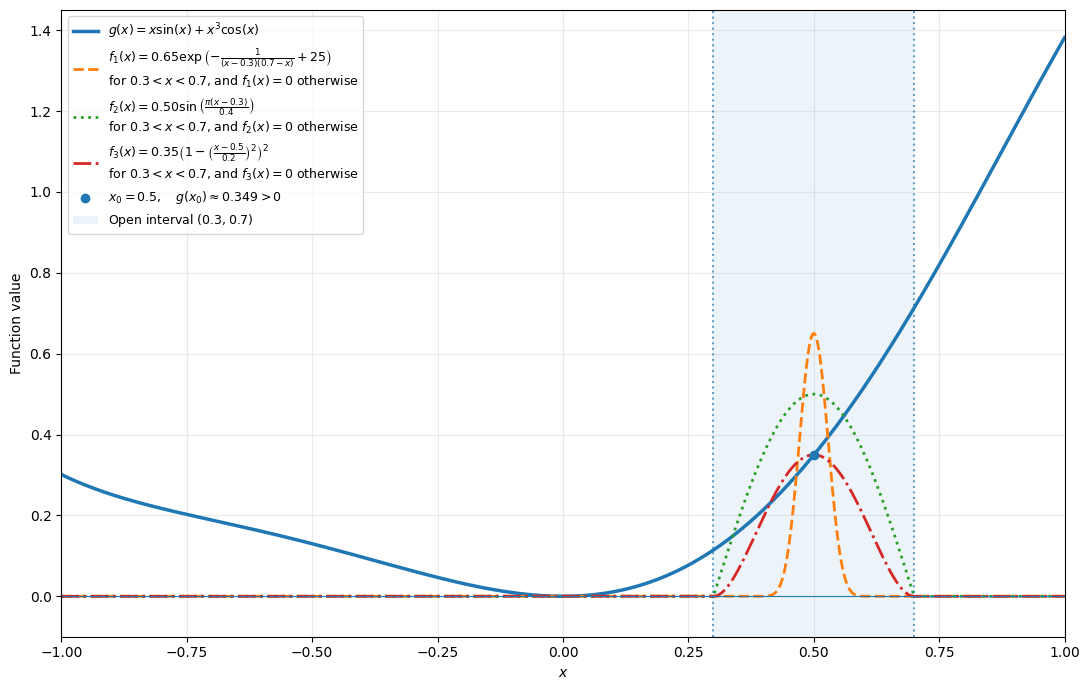
\includegraphics[scale=0.5]{images/bump_functions}
\caption{פונקציה
$g$
ושלוש דוגמאות לפונקציות שחיוביות על קטע פתוח סביב
$x_0 = 0.5$
ושוות לאפס מחוץ לקטע הפתוח.}
\label{figure:bump-functions}
\end{center}
\end{figure}

\begin{lemma}\label{lemma}
אם כל
$g \in W^\perp$
היא אי־חיובית, מתקיים
$W^\perp = \set{0}$.
\end{lemma}

\begin{proof}
תהי
$g \in W^\perp$
ויהי
$x \in \brs{-1,1}$.
אם
$g\prs{x} \neq 0$
נקבל מההנחה כי
$g\prs{x} < 0$.
אבל גם
$-g \in W^\perp$
מסגירות לכפל בסקלר, ואז
$\prs{-g}\prs{x} = -g\prs{x} > 0$
בסתירה לכך ש־%
$-g$
אי־חיובית.

לכן
$g\prs{x} = 0$
לכל
$x \in \brs{-1, 1}$.
\end{proof}

\begin{proposition}
מתקיים
$W^\perp = \set{0}$.
\end{proposition}

\begin{proof}
לפי למה
\ref{lemma}
די להראות כי כל
$g \in W^\perp$
היא אי־חיובית.

תהי
$g \in W^\perp$
ונוכיח כי
$g\prs{x} \leq 0$
לכל
$x \in \brs{-1, 1} \setminus \set{0}$.
אז מרציפות נקבל כי גם
$g\prs{x} \leq 0$
ולכן
$g$
אי־חיובית כנדרש.

תהי
$x_0 \in \brs{-1, 1}$
ונניח בדרך השלילה כי
$g\prs{x_0} > 0$.
מרציפות, קיימת
$\delta > 0$
כך שמתקיים
\begin{align} \label{equation}
\abs{g\prs{x} - g\prs{x_0}} < g\prs{x_0}
\end{align}
לכל
$x \in I \coloneqq \prs{x_0 - \delta, x_0 + \delta}$.
אם
$\delta \geq x_0$
ניקח במקום זאת את
$\delta' = \min\set{\delta, \frac{x_0}{2}}$
כך שמתקיים
\ref{equation}
גם לכל
$x \in I' \coloneqq \prs{x_0 - \delta', x_0 + \delta'}$.
לכן ניתן להניח בלי הגבלת הכלליות כי
$\delta < x_0$
ולכן
$0 \notin I$.
בנוסף, לכל
$x \in I$
מתקיים
\begin{align*}
g\prs{x_0} - g\prs{x} < g\prs{x_0}
\end{align*}
ולכן
\begin{align*}
g\prs{x} > 0
\end{align*}
ונקבל כי
$g$
חיובית על
$I$.

נגדיר
$f \colon \brs{-1, 1} \to \RR$
שהינה חיובית על
$I$
ושווה
$0$
מחוץ ל־%
$I$.
ניקח
\begin{align*}
\text{.} f\prs{x} = \fcases{\prs{1 - \prs{\frac{x - x_0}{\delta}}^2}^2 & x \in I \\ 0 & x \notin I}
\end{align*}
אז לכל
$x \in I$
מתקיים
\begin{align*}
\abs{\frac{x - x_0}{\delta}} = \frac{\abs{x - x_0}}{\delta} < \frac{\delta}{\delta} = 1
\end{align*}
ולכן
\begin{align*}
1 - \prs{\frac{x - x_0}{\delta}}^2 > 1 - 1^2 = 0
\end{align*}
ונקבל כי
\[\text{.} f\prs{} = \prs{1 - \prs{\frac{x - x_0}{\delta}}^2}^2 > 0\]

בנוסף
\begin{align*}
\prs{1 - \prs{\frac{\prs{x_0 \pm \delta} - x_0}{\delta}}^2}^2 = 0
\end{align*}
ולכן
$f$
רציפה. כיוון ש־%
$f$
מתאפסת מחוץ ל־%
$I$
ומתקיים
$0 \notin I$
נקבל כי
$f\prs{0} = 0$
ולכן
$f \in W$.

כיוון ש־%
$g \in W^\perp$
נקבל כי
\begin{align*}
\int_{-1}^1 g\prs{x} f\prs{x} \diff x = 0
\end{align*}
אבל
\begin{align*}
\int_{-1}^1 g\prs{x} f\prs{x} \diff x
&=
\int_I g\prs{x} f\prs{x} \diff x > 0
\end{align*}
כאשר האינטגרל השני חיובי כאינטגרל של פונקציה חיובית על קטע פתוח.

קיבלנו סתירה, ולכן
$g\prs{x_0} \leq 0$.
נקבל כי
$g$
אי־חיובית, כנדרש.
\end{proof}

\end{description}

\end{document}